\begin{ex}
	Rút gọn biểu thức: $A = \left( \frac{\sqrt{x}}{x-3\sqrt{x}} - \frac{1}{\sqrt{x}+3} \right) : \frac{3\sqrt{x}}{x-9}$ với $x>0$ và $x \neq 9$.
	\loigiai{
		Điều kiện: $x>0, x \neq 9$.
		Ta có:
		\begin{align*} A &= \left( \frac{\sqrt{x}}{\sqrt{x}(\sqrt{x}-3)} - \frac{1}{\sqrt{x}+3} \right) : \frac{3\sqrt{x}}{(\sqrt{x}-3)(\sqrt{x}+3)} \\ &= \left( \frac{1}{\sqrt{x}-3} - \frac{1}{\sqrt{x}+3} \right) \cdot \frac{(\sqrt{x}-3)(\sqrt{x}+3)}{3\sqrt{x}} \\ &= \left( \frac{(\sqrt{x}+3) - (\sqrt{x}-3)}{(\sqrt{x}-3)(\sqrt{x}+3)} \right) \cdot \frac{(\sqrt{x}-3)(\sqrt{x}+3)}{3\sqrt{x}} \\ &= \frac{\sqrt{x}+3 - \sqrt{x}+3}{(\sqrt{x}-3)(\sqrt{x}+3)} \cdot \frac{(\sqrt{x}-3)(\sqrt{x}+3)}{3\sqrt{x}} \\ &= \frac{6}{(\sqrt{x}-3)(\sqrt{x}+3)} \cdot \frac{(\sqrt{x}-3)(\sqrt{x}+3)}{3\sqrt{x}} \\ &= \frac{6}{3\sqrt{x}} \\ &= \frac{2}{\sqrt{x}} \end{align*}
		Vậy $A = \frac{2}{\sqrt{x}}$.
	}
\end{ex}

\begin{ex}
	Giải hệ phương trình sau:
	$$ \begin{cases} 3x-y=5 \\ 5x+2y=12 \end{cases} $$
	\loigiai{
		Ta có hệ phương trình:
		$$ \begin{cases} 3x-y=5 \quad &(1) \\ 5x+2y=12 \quad &(2) \end{cases} $$
		Nhân phương trình (1) với 2, ta được:
		$$ \begin{cases} 6x-2y=10 \quad &(1') \\ 5x+2y=12 \quad &(2) \end{cases} $$
		Cộng vế theo vế của phương trình (1') và (2), ta được:
		$(6x-2y) + (5x+2y) = 10 + 12$
		$11x = 22$
		$x = 2$.
		Thay $x=2$ vào phương trình (1):
		$3(2) - y = 5$
		$6 - y = 5$
		$y = 6 - 5$
		$y = 1$.
		Vậy nghiệm của hệ phương trình là $(x; y) = (2; 1)$.
	}
\end{ex}

\begin{ex}
	Cho phương trình: $2x^2-5x+1=0$. Tính giá trị của biểu thức: $T=(x_1-x_2)(x_1^2-x_2^2)$.
	\loigiai{
		Phương trình $2x^2-5x+1=0$ có $a=2, b=-5, c=1$.
		$\Delta = b^2-4ac = (-5)^2 - 4(2)(1) = 25 - 8 = 17 > 0$.
		Phương trình có hai nghiệm phân biệt $x_1, x_2$.
		Theo hệ thức Vi-ét, ta có:
		$$ \begin{cases} x_1 + x_2 = -\frac{b}{a} = -\frac{-5}{2} = \frac{5}{2} \\ x_1 x_2 = \frac{c}{a} = \frac{1}{2} \end{cases} $$
		Ta có $(x_1-x_2)^2 = (x_1+x_2)^2 - 4x_1x_2 = \left(\frac{5}{2}\right)^2 - 4\left(\frac{1}{2}\right) = \frac{25}{4} - 2 = \frac{25-8}{4} = \frac{17}{4}$.
		Do đó, $|x_1-x_2| = \frac{\sqrt{17}}{2}$.
		Giả sử $x_1 > x_2$, thì $x_1-x_2 = \frac{\sqrt{17}}{2}$. (Nếu $x_1 < x_2$ thì $x_1-x_2 = -\frac{\sqrt{17}}{2}$, nhưng $T$ sẽ không đổi dấu vì $(x_1-x_2)^2$ xuất hiện).
		
		Ta biến đổi biểu thức T:
		\begin{align*} T &= (x_1-x_2)(x_1^2-x_2^2) \\ &= (x_1-x_2)(x_1-x_2)(x_1+x_2) \\ &= (x_1-x_2)^2 (x_1+x_2) \end{align*}
		Thay các giá trị đã tính vào biểu thức T:
		\begin{align*} T &= \left(\frac{17}{4}\right) \cdot \left(\frac{5}{2}\right) \\ &= \frac{17 \cdot 5}{4 \cdot 2} \\ &= \frac{85}{8} \end{align*}
		Vậy $T = \frac{85}{8}$.
	}
\end{ex}
\begin{ex}
	Một chiếc hộp có chứa 5 tấm thẻ cùng loại, được đánh số lần lượt là 3; 5; 6; 7; 9. Lấy ngẫu nhiên đồng thời 2 tấm thẻ từ hộp. Tính xác suất của biến cố A: “Tích các số ghi trên 2 tấm thẻ chia hết cho 3”.
	\loigiai{
		Các tấm thẻ được đánh số: $\{3; 5; 6; 7; 9\}$.
		Lấy ngẫu nhiên đồng thời 2 tấm thẻ. Các cặp thẻ có thể lấy (không gian mẫu $\Omega$):
		$\Omega = \{ (3;5); (3;6); (3;7); (3;9); (5;6); (5;7); (5;9); (6;7); (6;9); (7;9) \}$.
		Số phần tử của không gian mẫu là $n(\Omega) = 10$.
		
		Biến cố A: “Tích các số ghi trên 2 tấm thẻ chia hết cho 3”.
		Để tích hai số chia hết cho 3 thì ít nhất một trong hai số đó phải chia hết cho 3.
		Các số chia hết cho 3 trong tập hợp đã cho là: $\{3; 6; 9\}$.
		Các cặp thẻ mà tích các số ghi trên đó chia hết cho 3 (kết quả thuận lợi cho A):
		\begin{itemize}
			\item Chọn thẻ có số 3: $(3;5)$; $(3;6)$; $(3;7)$; $(3;9)$. (Tích: 15; 18; 21; 27)
			\item Chọn thẻ có số 6 (không lặp lại các cặp đã có số 3): $(5;6)$; $(6;7)$; $(6;9)$. (Tích: 30; 42; 54)
			\item Chọn thẻ có số 9 (không lặp lại các cặp đã có số 3 hoặc 6): $(5;9)$; $(7;9)$. (Tích: 45; 63)
		\end{itemize}
		Vậy, $A = \{ (3;5); (3;6); (3;7); (3;9); (5;6); (5;9); (6;7); (6;9); (7;9) \}$.
		Số phần tử của biến cố A là $n(A) = 9$.
		
		Xác suất của biến cố A là:
		$P(A) = \frac{n(A)}{n(\Omega)} = \frac{9}{10}$.
	}
\end{ex}
\begin{ex}
	Một tàu thủy chạy trên một khúc sông dài 80km. Cả đi lẫn về hết 8h20p. Tính tốc độ của tàu thủy khi nước yên lặng biết tốc độ dòng nước là 4km/h.
	\loigiai{
		Gọi tốc độ của tàu thủy khi nước yên lặng là $x$ (km/h).
		Điều kiện: $x > 4$ (vì tốc độ tàu phải lớn hơn tốc độ dòng nước để có thể đi ngược dòng).
		
		Đổi 8 giờ 20 phút = $8 + \frac{20}{60}$ giờ = $8 + \frac{1}{3}$ giờ = $\frac{25}{3}$ giờ.
		
		Tốc độ của tàu thủy khi đi xuôi dòng là: $x + 4$ (km/h).
		Thời gian tàu thủy đi xuôi dòng 80km là: $\frac{80}{x+4}$ (giờ).
		
		Tốc độ của tàu thủy khi đi ngược dòng là: $x - 4$ (km/h).
		Thời gian tàu thủy đi ngược dòng 80km là: $\frac{80}{x-4}$ (giờ).
		
		Vì tổng thời gian cả đi lẫn về là $\frac{25}{3}$ giờ, ta có phương trình:
		$$ \frac{80}{x+4} + \frac{80}{x-4} = \frac{25}{3} $$
		Quy đồng mẫu số và giải phương trình:
		\begin{align*}
			80 \cdot 3 (x-4) + 80 \cdot 3 (x+4) &= 25 (x+4)(x-4) \\
			240(x-4) + 240(x+4) &= 25(x^2 - 16) \\
			240x - 960 + 240x + 960 &= 25x^2 - 400 \\
			480x &= 25x^2 - 400 \\
			25x^2 - 480x - 400 &= 0
		\end{align*}
		Chia cả hai vế cho 5:
		$$ 5x^2 - 96x - 80 = 0 $$
		Giải phương trình bậc hai $5x^2 - 96x - 80 = 0$:
		Ta có $\Delta' = b'^2 - ac = (-48)^2 - 5(-80) = 2304 + 400 = 2704$.
		$\sqrt{\Delta'} = \sqrt{2704} = 52$.
		Phương trình có hai nghiệm phân biệt:
		$x_1 = \frac{-b' + \sqrt{\Delta'}}{a} = \frac{48 + 52}{5} = \frac{100}{5} = 20$.
		$x_2 = \frac{-b' - \sqrt{\Delta'}}{a} = \frac{48 - 52}{5} = \frac{-4}{5}$.
		
		Đối chiếu với điều kiện $x > 4$:
		Nghiệm $x_1 = 20$ (thỏa mãn).
		Nghiệm $x_2 = -\frac{4}{5}$ (không thỏa mãn).
		
		Vậy, tốc độ của tàu thủy khi nước yên lặng là 20 km/h.
	}
\end{ex}
\begin{ex}
	Cho $\triangle ABC$ có ba góc nhọn nội tiếp đường tròn (O) và $AB < AC$. Kẻ đường cao AD của tam giác ABC và đường kính AE của đường tròn tâm (O). Gọi F là chân đường vuông góc kẻ từ B xuống đường kính AE.
	\begin{enumerate}
		\item[a)] Chứng minh: bốn điểm A; B; D; F cùng thuộc một đường tròn.
		\item[b)] Chứng minh: $AB \cdot AC = AD \cdot AE$ và DF vuông góc với AC.
	\end{enumerate}
	\loigiai{
	\begin{center}
		
		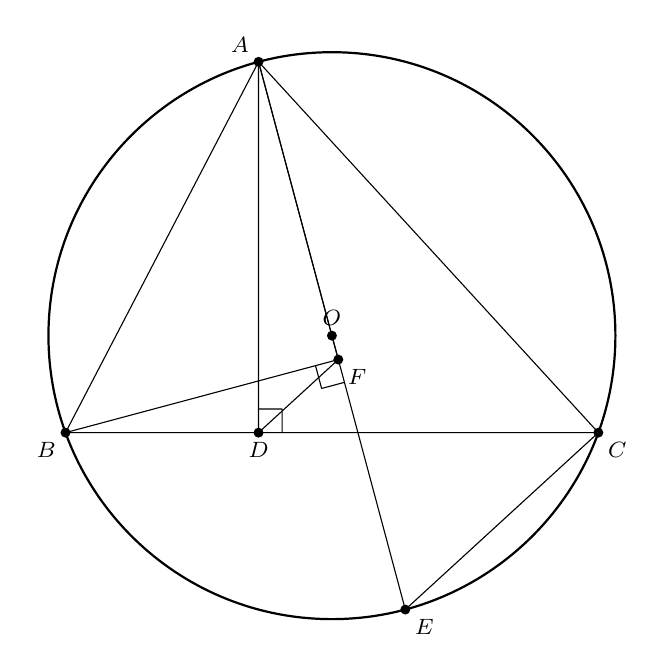
\begin{tikzpicture}[line join = round, line cap=round,>=stealth,font=\footnotesize,scale=1.2]
			\usetikzlibrary{calc,angles,quotes} % quotes for potential future use with angle labels
			% Def
			\def\r{3}
			
			% Coordinates
			\coordinate (O) at (0,0);
			\coordinate (B) at (-160:\r); % Điểm B
			\coordinate (C) at (-20:\r);  % Điểm C
			\coordinate (A) at (105:\r);  % Điểm A
			
			% D là hình chiếu của A lên BC
			\coordinate (D) at ($ (B)!(A)!(C) $);
			
			% E sao cho O là trung điểm của AE
			% E là điểm đối xứng của A qua O
			\coordinate (E) at ($ 2*(O) - (A) $); 
			% Hoặc \coordinate (E) at (105+180:\r);
			
			% F là hình chiếu của B lên AE
			\coordinate (F) at ($ (A)!(B)!(E) $);
			
			% Draw
			% Vẽ đường tròn (O,r)
			\draw[thick] (O) circle (\r);
			
			% Vẽ các đường A-B-C-A
			\draw (A) -- (B) -- (C) -- cycle;
			
			% Vẽ A-D
			\draw (A) -- (D);
			
			% Vẽ D-F
			\draw (D) -- (F);
			
			% Vẽ F-B
			\draw (F) -- (B);
			
			% Vẽ F-A (đoạn này là một phần của AE)
			\draw (F) -- (A); % Thực ra đã được bao gồm nếu vẽ AE, nhưng để rõ ràng
			
			% Vẽ A-E
			\draw (A) -- (E);
			
			% Vẽ E-C
			\draw (E) -- (C);
			
			% Fill points
			\fill (O) circle (1.5pt);
			\fill (A) circle (1.5pt);
			\fill (B) circle (1.5pt);
			\fill (C) circle (1.5pt);
			\fill (D) circle (1.5pt);
			\fill (E) circle (1.5pt);
			\fill (F) circle (1.5pt);
			
			% Node points (old style)
			\node[above] at (O) {$O$};
			\node[above left] at (A) {$A$};       % A ở góc phần tư II
			\node[below left] at (B) {$B$};       % B ở góc phần tư III
			\node[below right] at (C) {$C$};      % C ở góc phần tư IV
			\node[below] at (D) {$D$};            % D trên BC
			\node[below right] at (E) {$E$};      % E ở góc phần tư IV (đối xứng A qua O)
			\node[below right] at (F) {$F$}; % F trên AE, vị trí tương đối
			
			% Ký hiệu góc vuông (old style)
			% AD vuông góc BC
			\pic[draw, angle radius=3mm]{right angle = A--D--C}; % Giả sử D nằm giữa B và C, hoặc gần C
			% BF vuông góc AE
			\pic[draw, angle radius=3mm]{right angle = B--F--E}; % Giả sử F nằm giữa A và E
			
		\end{tikzpicture}
		
	
	\end{center}
	
	}
\end{ex}

\begin{ex}
	Cho a, b, c là các số thực dương thoả mãn: $a+b+c=3$. Tìm giá trị nhỏ nhất của biểu thức:
	$$ P = \frac{2024}{\sqrt{ab}+\sqrt{bc}+\sqrt{ac}} + \frac{b\sqrt{a}}{1+b} + \frac{c\sqrt{b}}{1+c} + \frac{a\sqrt{c}}{1+a} $$
\end{ex}

\setcounterref{ex}{0}
